% !TeX root = template.tex
%!BIB program = bibtex
%%%%%%%%%%%%%%%%%%%%%%% file template.tex %%%%%%%%%%%%%%%%%%%%%%%%%
%
% This is a template file for the LaTeX package SVJour2 for the
% Springer journal "Machine Vision and Applications".
%
%                                    Springer Heidelberg 2004/11/04
%
% Copy it to a new file with a new name and use it as the basis
% for your article. Delete % as needed.
%
%%%%%%%%%%%%%%%%%%%%%%%%%%%%%%%%%%%%%%%%%%%%%%%%%%%%%%%%%%%%%%%%%%%
%
% First comes an example EPS file -- just ignore it and
% proceed on the \documentclass line
% your LaTeX will extract the file if required
\begin{filecontents*}{example.eps}
%!PS-Adobe-3.0 EPSF-3.0
%%BoundingBox: 19 19 221 221
%%CreationDate: Mon Sep 29 1997
%%Creator: programmed by hand (JK)
%%EndComments
gsave
newpath
  20 20 moveto
  20 220 lineto
  220 220 lineto
  220 20 lineto
closepath
2 setlinewidth
gsave
  .4 setgray fill
grestore
stroke
grestore
\end{filecontents*}
%
\documentclass[twocolumn,fleqn,runningheads]{svjour2}
%
\smartqed  % flush right qed marks, e.g. at end of proof
%
\usepackage{graphicx}
\usepackage{biograph} 
\usepackage{mwe}
\usepackage{subfig}       % to allow for author biography at the end
%
%\usepackage{mathptmx}      % use Times fonts if available on your TeX system
%
% insert here the call for the packages your document requires
%\usepackage{latexsym}
% etc.
%
% please place your own definitions here and don't use \def but
% \newcommand{}{}
%
\journalname{Machine Vision and Applications}
%
\begin{document}

\title{Zelda Music Generation using a RNN%\thanks{Grants or other notes
%about the article that should go on the front page should be
%placed here. General acknowledgments should be placed at the end of the article.}
}
\subtitle{idk what subtitle}

%\titlerunning{Short form of title}        % if too long for running head

\author{Tim Luecking}

%\authorrunning{Short form of author list} % if too long for running head

\institute{Tim Luecking \at
              Tulpenstrasse 6, 33181 Bad Wuennenberg \\
              Tel.: +49 15128743541
              \email{tim.luecking1@fh-bielefeld.de}   
}

\date{Received: 27.06.2022 / Accepted: date}
% The correct dates will be entered by the editor


\maketitle

\begin{abstract}
ABstract kommt hier hin....... was schreibt man da

\keywords{Zelda \and LSTM \and RNN \and Music \and Generation}
\end{abstract}

\section{Introduction}
\label{intro}

Great musicians like Beethoven died before they could finish their last work. The legacy
of Beethoven were 40 sketches for a 10th symphony. The project "Beethoven X - The AI 
Project" used AI to complete the 10th symphony using those sketches in a style that
mimics the ingenuity of Beethoven ~\cite{test:1}.

Projects like these are the best example for a usecase for AI generated music. It is not
only possible to complete given note sequences, but also to generate completly new 
melodies by using AI.

The beloved game series called "Zelda" by Nintendo comes with a big amount of nostalgic
melodies and songs. To create new melodies in the style of those games, an AI should be
trained to learn how the melodies are constructed. The goal is to let the AI generate
music notes and a new melody.

\section{Training Data}
\label{trainingdata}

To train the AI, music files in any form are needed. Single instrument
midi files are an easy way to train said AI. Midi (Musical Instrument Digital
Interface) is a technical standard that describes a communication protocoll
among other things to connect a wide variety of music instruments and other
audio devices. It is used to play, edit and record music. The length, the
velocity and frequency of each note is saved in a textual file format.

Midi files are an easy way to train an AI because of the numeric structure
of the files. Websites like "BitMidi" ~\cite{test:2} offer a wide variaty 
of free Midi files to download. 65 Single instrument songs from Zelda games 
were downloaded and will be used hereinafter as the training data of the AI.
In Figure ~\ref{fig:fullSong} is one of those midi songs displayed.

\begin{figure}
\centering
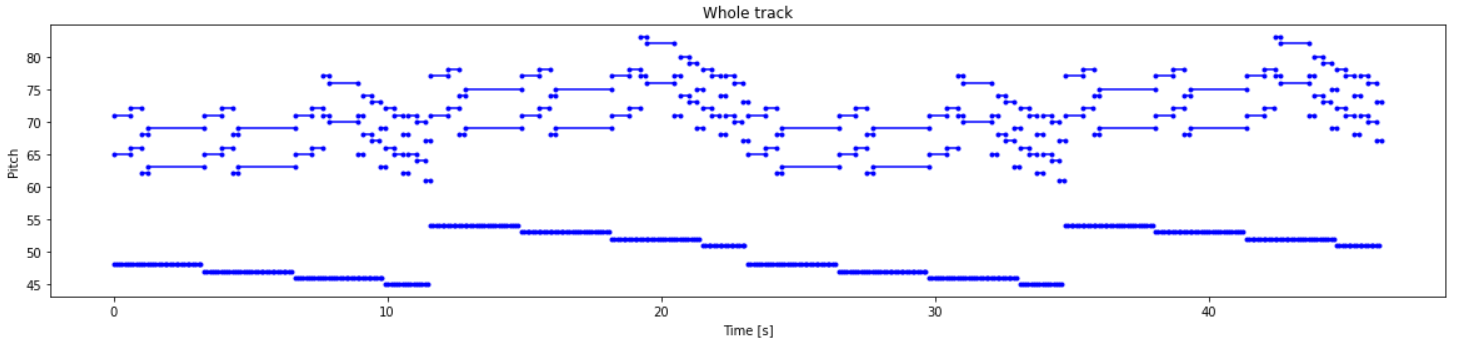
\includegraphics[width=0.5\textwidth]{./pics/fullSong.PNG}
\caption{Full Midi Sonng - "The Legend of Zelda - Death Mountain"}
\label{fig:fullSong}    
\end{figure}

All music files need to be read and changed by the program to acquire
a dataset for the neural network. A Long Short-Term Memory (LSTM) neural
network should be used to generate new melodies. A LSTM network is able to 
make predictions depending on a sequence of data. In terms of music this 
might mean that it can predict the next note by using a given sequence of 
multiple notes, that were played before.

With the help of the library "PrettyMidi" the Midi data is handled. All notes
from every Midi file is read and saved into an array. This array of tupels 
consists of the the pitch, the duration and the step of each note (step meaning
the length of the pause between the note and the note being played before).

Figure ~\ref{fig:verteilung} shows the distribution of pitch, step and duration
of all notes in the song "The Legend of Zelda - Death Mountain". The usage of 
low notes in contrast to really high notes is one of the key elements of 
the music of the Zelda games. Furthermore you can see, that the duration of
the notes are mostly short with only some outlier. 

\begin{figure}

\begin{minipage}{.5\linewidth}
\centering
\subfloat[]{\label{fig:test1}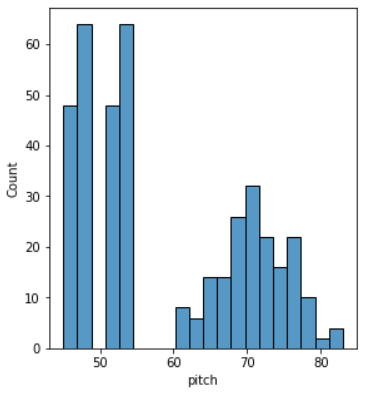
\includegraphics[scale=.5]{./pics/pitch.PNG}}
\end{minipage}%
\begin{minipage}{.5\linewidth}
\centering
\subfloat[]{\label{fig:test2}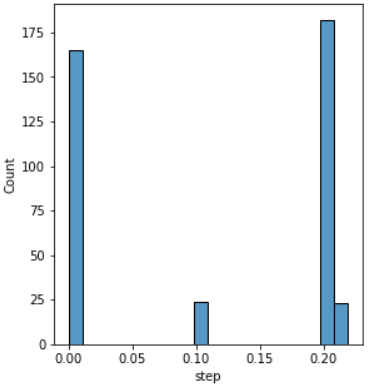
\includegraphics[scale=.5]{./pics/step.PNG}}
\end{minipage}\par
\centering
\subfloat[]{\label{fig:test3}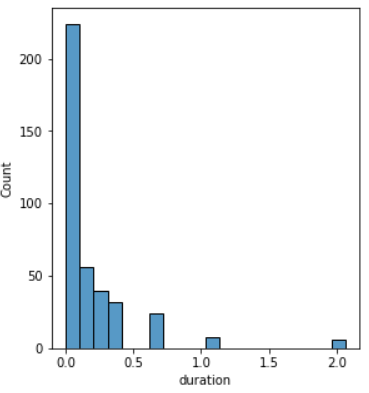
\includegraphics[scale=.5]{./pics/duration.PNG}}

\caption{Distribution of pitch, step and duration of "The Legend of Zelda - Death Mountain"}
\label{fig:verteilung}   
\end{figure}







- grundlagen\\
- datensatz\\
- wie wird der datensatz aufbereitet\\
- wie wierd dsa modell aufgebaut\\
- ausfuehren\\
- loss funktion\\
- verteilung noten vorher nachher\\
- conclusion\\

\section{Section title}
\label{sec:1}
%%Citations \cite{Ref1} and \cite{Ref2} and \cite{Ref3}.
\subsection{Subsection title}
\label{sec:2}
as required. Don't forget to give each section
and subsection a unique label (see Sect.~\ref{sec:1}).
\paragraph{Paragraph headings} Use paragraph headings as needed.
\begin{equation}
a^2+b^2=c^2
\end{equation}

% For one-column wide figures use
\begin{figure}
\centering
% Use the relevant command to insert your figure file.
% For example, with the graphicx package use
  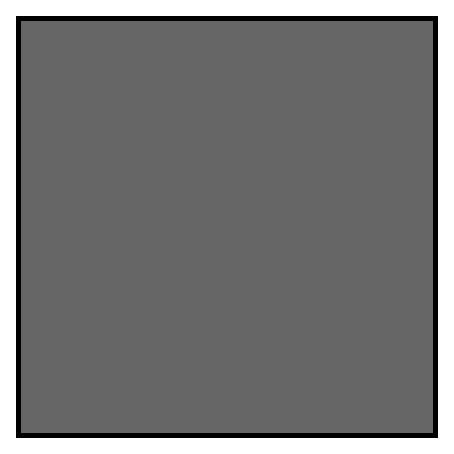
\includegraphics{example.eps}
% figure caption is below the figure
\caption{Please write your figure caption here}
\label{fig:1}       % Give a unique label
\end{figure}
%
% For two-column wide figures use
\begin{figure*}
\centering
% Use the relevant command to insert your figure file.
% For example, with the graphicx package use
  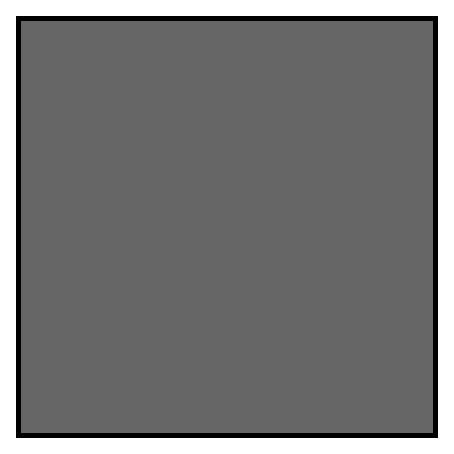
\includegraphics[width=0.75\textwidth]{example.eps}
% figure caption is below the figure
\caption{Please write your figure caption here}
\label{fig:2}       % Give a unique label
\end{figure*}
%
% For tables use
\begin{table}[t]
% table caption is above the table
\caption{Please write your table caption here}
\centering
\label{tab:1}       % Give a unique label
% For LaTeX tables use
\begin{tabular}{lll}
\hline\noalign{\smallskip}
first & second & third  \\[3pt]
\tableheadseprule\noalign{\smallskip}
number & number & number \\
number & number & number \\
\noalign{\smallskip}\hline
\end{tabular}
\end{table}


%\begin{acknowledgements}
%If you'd like to thank anyone, place your comments here
%and remove the percent signs.
%\end{acknowledgements}

% BibTeX users please use
\bibliographystyle{spmpsci}
\bibliography{zelda}   % name your BibTeX data base

% Non-BibTeX users please use
%\begin{thebibliography}{3}
%
% and use \bibitem to create references. Consult the Instructions
% for authors for reference list style.\cite{test:1}
%
% Format for Journal Reference
%\bibitem{Ref1}
%Author, I.: Article title. Journal Title-Abbreviated {\bf Vol}, pp--pp (year)
%% Format for books
%\bibitem{Ref2}
%Author, I., Smith, J.: Book Title. Publisher, Place (year)
% Format for proceedings
%\bibitem{Ref3}
%%Author, I., Smith, J.: Paper title. In: Editor, A. (ed.) Proceedings
%Title, Location, Date, pages. Publisher, Place (year)
% etc
%\end{thebibliography}

\begin{authorbiography}{example.eps}{A.N. Author}\
biography will be printed here if needed. Whether an author
biography is included per author is set
per journal. A photo is optional.
\end{authorbiography}

\end{document}
% end of file template.tex
